\newpage
\section{Auswertung}
\label{sec:evaluation}
Die aufgenommenen Photolumineszenzspektren für alle vier untersuchten Proben sind in Abbildung \ref{fig:Pol0}
dargestellt. 
\subsection{Bestimmung der Größe der Nanokristalle}
\begin{figure}[H]
    \centering
    \begin{subfigure}{0.49\textwidth}
        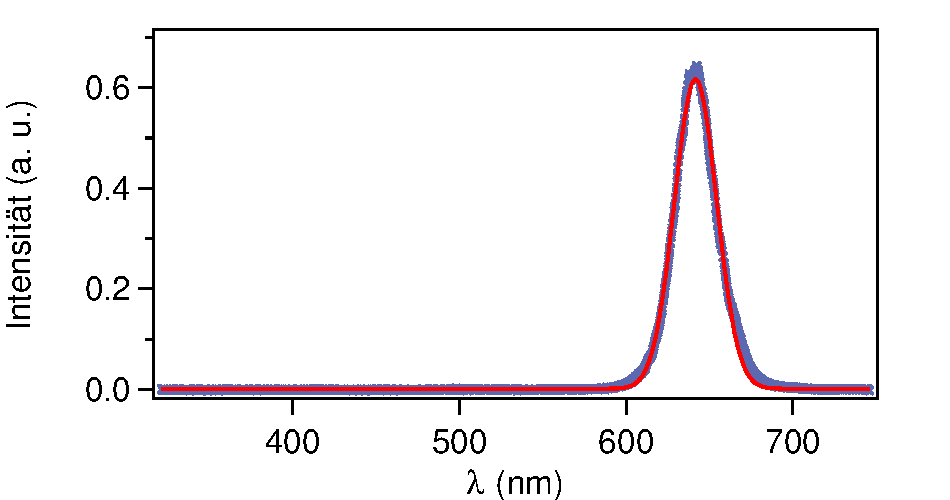
\includegraphics[width=\textwidth]{bilder/N1_Pol0.pdf}
        \caption{}
        \label{fig:A1}
    \end{subfigure}
    \begin{subfigure}{0.49\textwidth}
        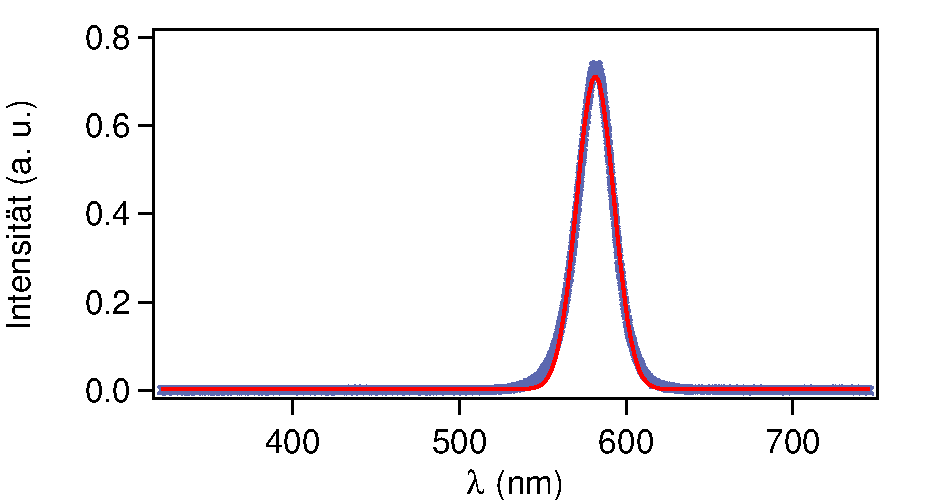
\includegraphics[width=\textwidth]{bilder/Nr2_Pol0.pdf}
        \caption{}
        \label{fig:A2}
    \end{subfigure}
    \begin{subfigure}{0.49\textwidth}
        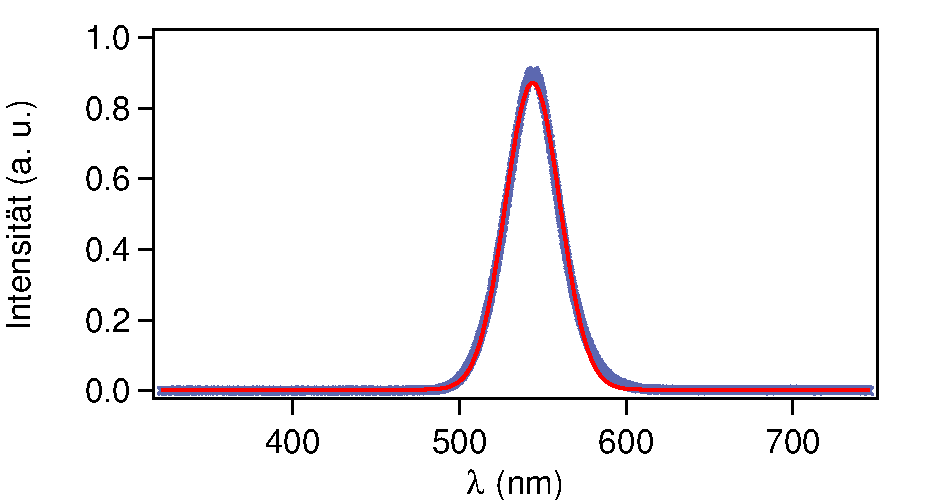
\includegraphics[width=\textwidth]{bilder/Nr3_Pol0.pdf}
        \caption{}
        \label{fig:A3}
    \end{subfigure}
    \begin{subfigure}{0.49\textwidth}
        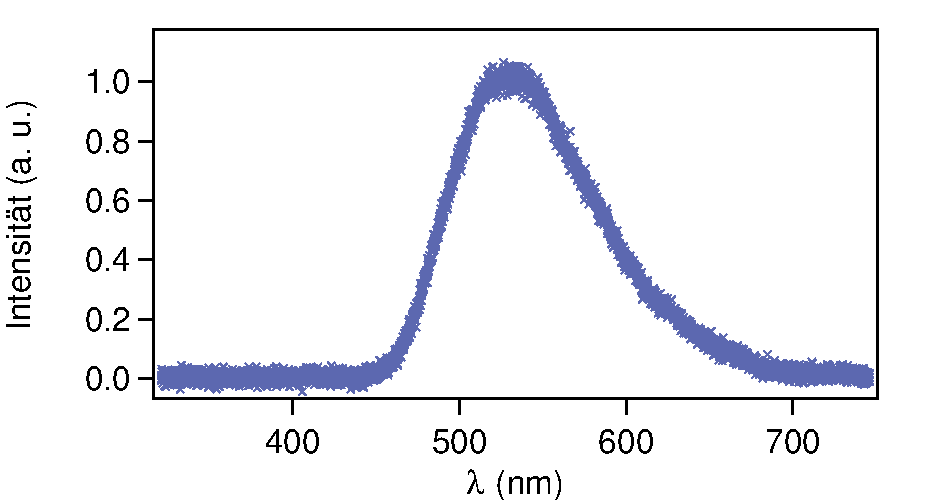
\includegraphics[width=\textwidth]{bilder/Nr4_Pol0.pdf}
        \caption{}
        \label{fig:A4}
    \end{subfigure}
    \caption{Photolumineszenzspektren der untersuchten Proben bei einer Polarisation von 0°. Dabei zeigen \textbf{(a)-(d)} jeweils Proben Nr.1 bis Nr.4. Für die Größenbestimmung der Nanokristalle wurden Gaußfits an die Spektren \textbf{(a)-(c)} angepasst.}
    \label{fig:Pol0}
\end{figure}
Für die Kristallgrößenbestimmung wurden Gaußfits angelegt um die genaue Peakposition zu ermitteln.
Die Kristallgröße wurde mittels \autoref{eqn:PL_formel} errechnet, dabei wurde $\epsilon_{\text{r}}=9,5$, $\frac{m_e^*}{m_{\text0}}=0,13$, $\frac{m_h^*}{m_{\text0}}=0,45$ und $E_{\text{G}=1,74\,\si{\electronvolt}}$ genutzt (siehe \cite{anleitung}, \cite{Manipulation}).

\begin{table}[H]
    \centering
    \makebox[\textwidth][c]{
    \begin{tabular}{c c c}
    \toprule
    Probe & Peakposition [nm] & Kristallgröße [nm] \\
    \midrule
    Nr.1 & $641.771\pm0,018$ & $2.4892\pm0,0007$\\
    Nr.2 & $581.632\pm0,014$ & $1.9338\pm0,0004$\\
    Nr.3 & $544.061\pm0,015$ & $1.8023\pm0,0004$\\
    \bottomrule
    \end{tabular}
    }
    \caption{Mittels Gaußfit bestimmte Peakpositionen und errechnete Kristallgrößen für die Nanokristalle.}
    \label{tab:Kristallgroesse}
\end{table}

\subsection{Polarisation}
Die Polarisation $P$ wird nach der Formel

\begin{equation}
    P=\frac{I_{0\,°}-I_{90\,°}}{I_{0\,°}+I_{90\,°}}
\end{equation}
berechnet. Die gemessenen Intensitäten zusammen mit der errechneten Polarisation sind in Tabelle \ref{tab:Pol} aufgelistet.


\begin{table}[H]
    \centering
    \makebox[\textwidth][c]{
    \begin{tabular}{c c c c}
    \toprule
    Probe & $I_{0\,°}$ & $I_{90\,°}$ & $P$ \\
    \midrule
    Nr.1 & $0,6144\pm0,0008$ & $0,61438\pm0,00015$ & $0,0000\pm0,0006$\\
    Nr.2 & $0,7097\pm0,0008$ & $0,7056\pm0,0008$& $0,0029\pm0,0008$\\
    Nr.3 & $0,8682\pm0,0007$ & $0,8662\pm0,0007$& $0,0012\pm0,0006$\\
    Nr.4 & $1,0043\pm0,0029$ & $0,9932\pm0,0028$& $0,0050\pm0,0021$\\
    \bottomrule
    \end{tabular}
    }
    \caption{Aufgenommene Intensitäten und berechnete Polarisation für alle vermessenen Proben.}
    \label{tab:Pol}
\end{table}



\subsection{Abhängigkeit von der Laserleistung}
Die Emissionspeaks und -intensitäten sind für Probe Nr.3 für unterschiedliche Laserleistungen in Abbildung \ref{fig:Leistung} aufgetragen. 
Die Peakintensität hat eine lineare Abhängigkeit, die Peakposition jedoch weist keine Abhängigkeit von der Laserlsitung auf.
\begin{figure}[H]
    \centering
    \begin{subfigure}{0.375\textwidth}
        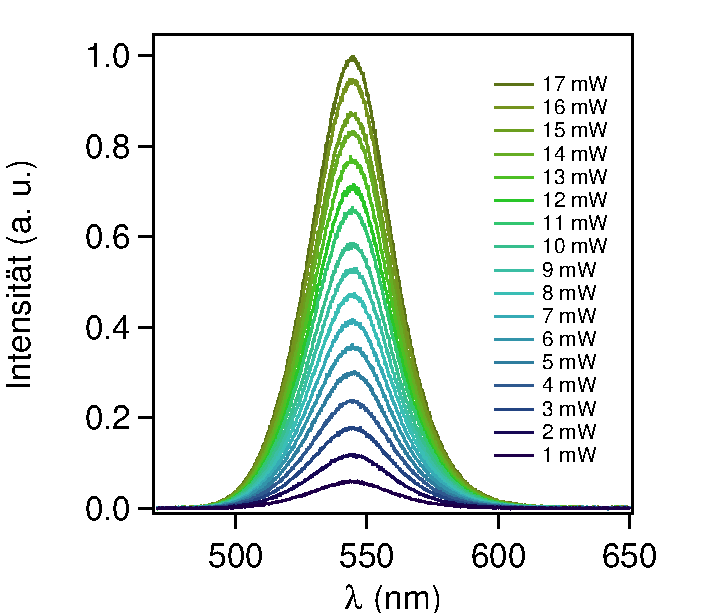
\includegraphics[width=\textwidth]{bilder/A2_Int.pdf}
        \caption{}
        \label{fig:A1}
    \end{subfigure}
    \begin{subfigure}{0.6\textwidth}
        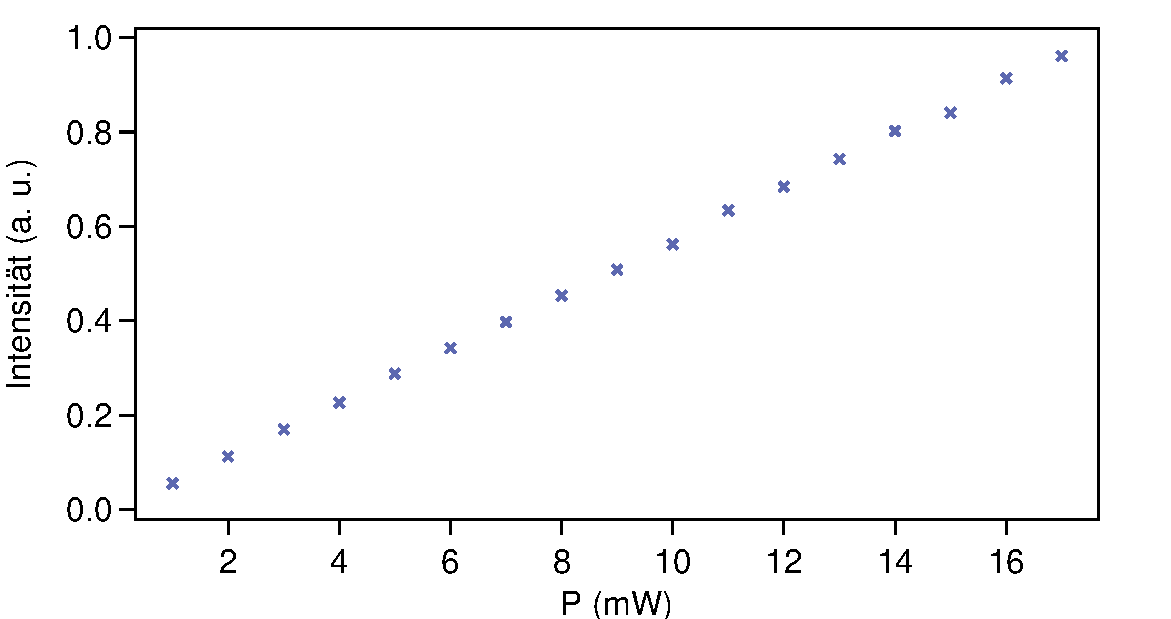
\includegraphics[width=\textwidth]{bilder/Int.pdf}
        \caption{}
        \label{fig:A2}
    \end{subfigure}
    \caption{\textbf{(a)} Photolumineszenzspektren um den Emissionspeak für verschiedene Laserleistungen. \textbf{(b)} Peakintensitäten in Abhängigkeit der Laserleistung.}
    \label{fig:Leistung}
\end{figure}
\subsection{Abhängigkeit von der Laseranregungswellenlänge}
Die Photolumineszenzspektren für verschiedene Laseranregungswellenlängen sind in Abbildung \ref{fig:Laserwellenlänge} aufgetragen.
\begin{figure}[H]
    \centering
    \begin{subfigure}{0.49\textwidth}
        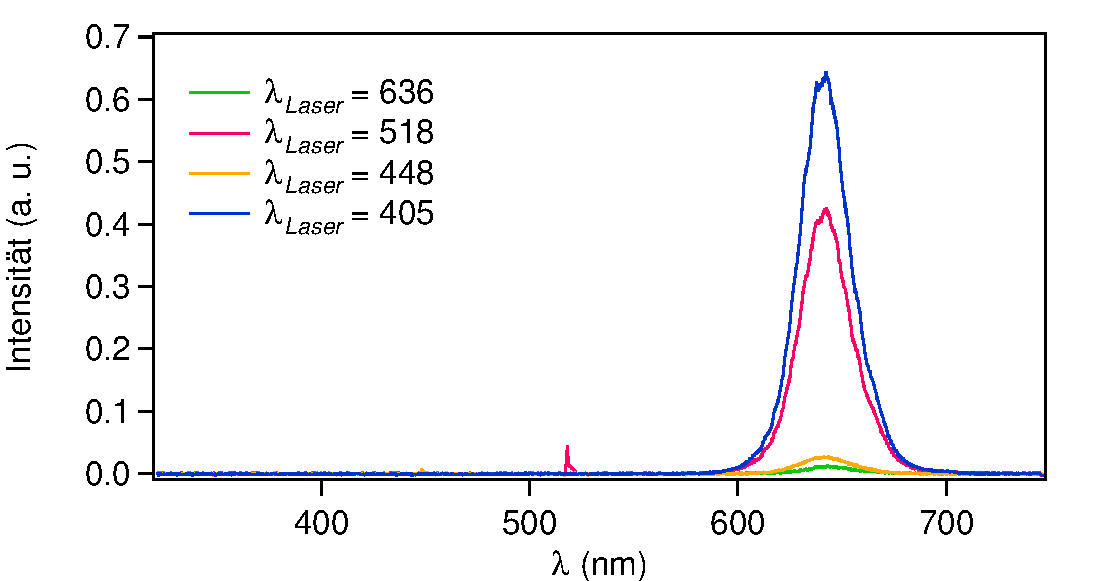
\includegraphics[width=\textwidth]{bilder/Nr1_Laser.pdf}
        \caption{}
        \label{fig:A1}
    \end{subfigure}
    \begin{subfigure}{0.49\textwidth}
        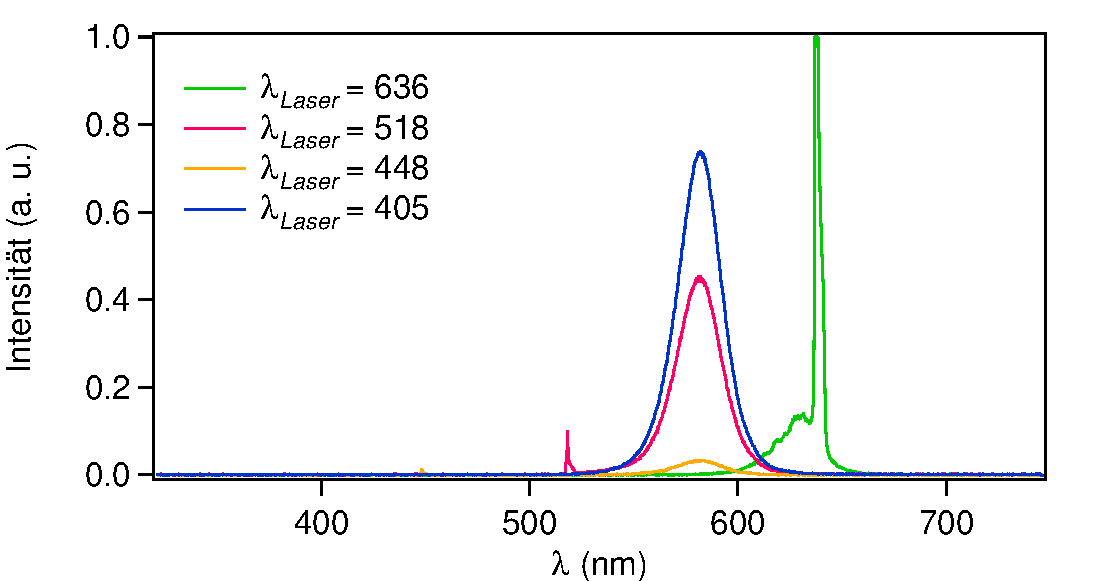
\includegraphics[width=\textwidth]{bilder/Nr2_Laser.pdf}
        \caption{}
        \label{fig:A2}
    \end{subfigure}
    \begin{subfigure}{0.49\textwidth}
        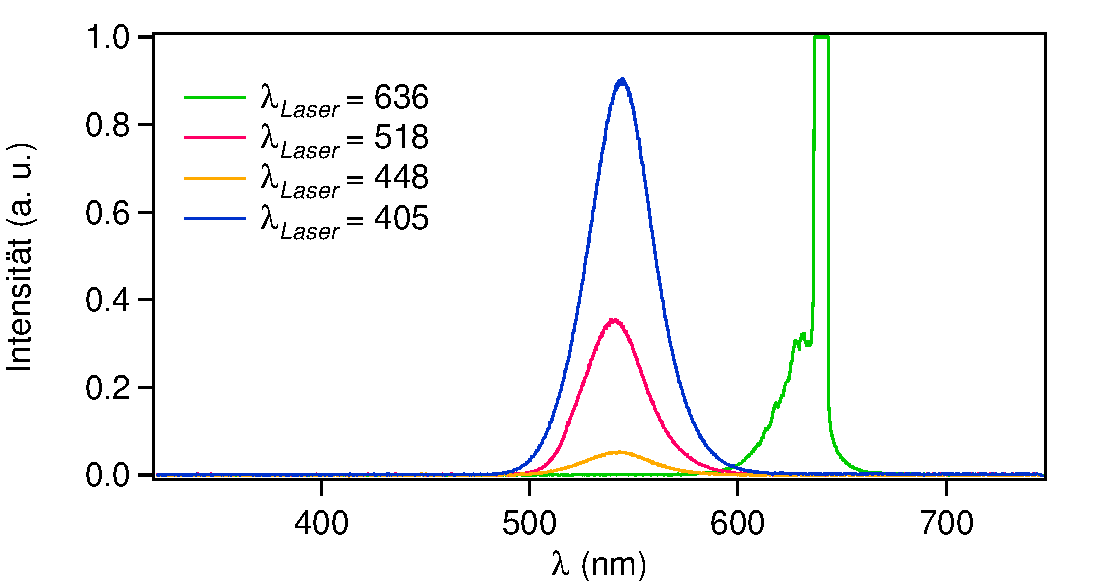
\includegraphics[width=\textwidth]{bilder/Nr3_Laser.pdf}
        \caption{}
        \label{fig:A3}
    \end{subfigure}
    \begin{subfigure}{0.49\textwidth}
        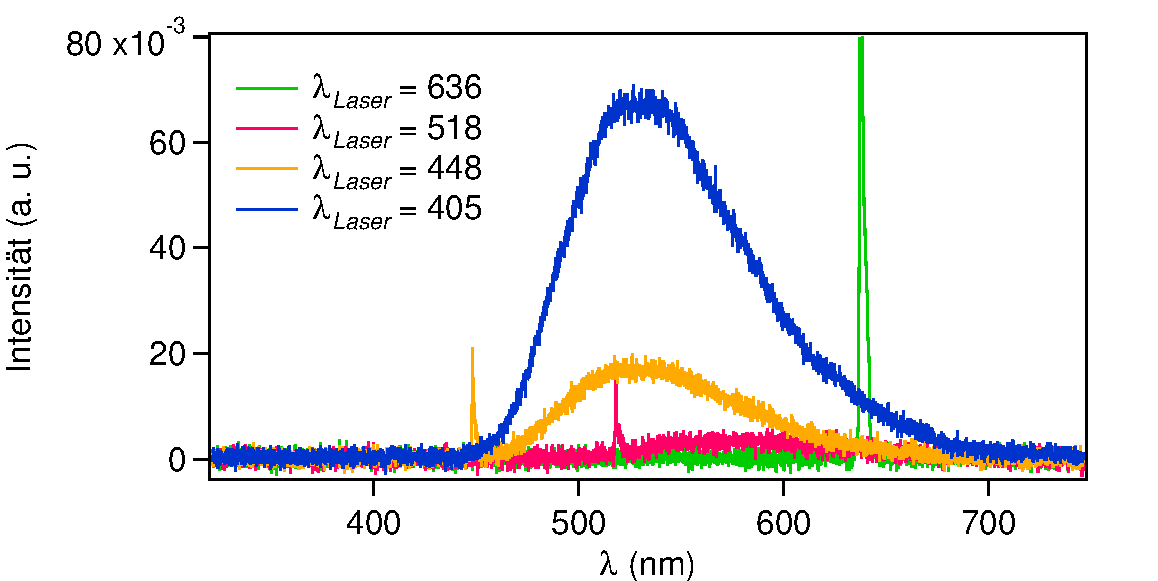
\includegraphics[width=\textwidth]{bilder/Nr4_Laser.pdf}
        \caption{}
        \label{fig:A4}
    \end{subfigure}
    \caption{Photolumineszenzspektren der untersuchten Proben für verschiedene Laseranregungswellenlängen.}
    \label{fig:Laserwellenlänge}
\end{figure}


Die schmalen Peaks (gerade beim $\lambda=636\,\si{\nano\meter}$-Laser)
sind auf Anteile des Laserlichts zurückzuführen, die direkt in den Detektor fallen.
Der $\lambda=636\,\si{\nano\meter}$-Laser erzeugt zudem nur bei der ersten Probe ein detektierbares Photolumineszenz-Signal.
Der $\lambda=518\,\si{\nano\meter}$-Laser und der $\lambda=448\,\si{\nano\meter}$-Laser
erzeugen jeweils schwächere Photolumineszenzpeaks, als der $\lambda=405\,\si{\nano\meter}$-Laser,
abgesehen von Probe Nr.4, wo nur letztere beiden Laser ein Signal hervorrufen.


